\documentclass[12pt]{article}
\usepackage[english]{babel}
\usepackage[utf8]{inputenc}

%% Pointer to 'default' preamble, other reusable files
% pacakages and definitions

\usepackage{geometry}
\geometry{
	letterpaper, 
	portrait, 
	top=.75in,
	left=.8in,
	right=.75in,
	bottom=.5in		} 	% Page Margins
	
%% additional packages for nice things
\usepackage{amsmath} 	% for most math
\usepackage{commath} 	% for abs
\usepackage{lastpage}	% for page count
\usepackage{amssymb} 	% for therefore
\usepackage{graphicx} 	% for image handling
\usepackage{wrapfig} 	% wrap figures
\usepackage[none]{hyphenat} % for no hyphenations
\usepackage{array} 		% for >{} column characterisctis
\usepackage{physics} 	% for easier derivative \dv....
\usepackage{tikz} 		% for graphic@!
\usepackage{circuitikz} % for circuits!
\usetikzlibrary{arrows.meta} % for loads
\usepackage[thicklines]{cancel}	% for cancels
\usepackage{xcolor}		% for color cancels
\usepackage[per-mode=fraction]{siunitx} % for si units and num
\sisetup{group-separator = {,}, group-minimum-digits = 3} % additional si unit table functionality

\usepackage{fancyhdr} 	% for header
\usepackage{comment}	% for ability to comment out large sections
\usepackage{multicol}	% for multiple columns using multicols
\usepackage[framed,numbered]{matlab-prettifier} % matlab sytle listing
\usepackage{marvosym} 	% for boltsymbol lightning
\usepackage{pdflscape} 	% for various landscape pages in portrait docs.
%\usepackage{float}
\usepackage{fancyvrb}	% for Verbatim (a tab respecting verbatim)
\usepackage{enumitem}	% for [resume] functionality of enumerate
\usepackage{spreadtab} 	% for using formulas in tables}
\usepackage{numprint}	% for number format in spread tab
\usepackage{subcaption} % for subfigures with captions
\usepackage[normalem]{ulem} % for strike through sout

% for row colors in tables....
\usepackage{color, colortbl}
\definecolor{G1}{gray}{0.9}
\definecolor{G2}{rgb}{1,0.88,1}%{gray}{0.6}
\definecolor{G3}{rgb}{0.88,1,1}

% For table formatting
\usepackage{booktabs}
\renewcommand{\arraystretch}{1.2}
\usepackage{floatrow}
\floatsetup[table]{capposition=top} % put table captions on top of tables

% Caption formating footnotesize ~ 10 pt in a 12 pt document
\usepackage[font={small}]{caption}

%% package config 
\sisetup{output-exponent-marker=\ensuremath{\mathrm{E}}} % for engineer E
\renewcommand{\CancelColor}{\color{red}}	% for color cancels
\lstset{aboveskip=2pt,belowskip=2pt} % for more compact table
%\arraycolsep=1.4pt\def
\setlength{\parindent}{0cm} % Remove indentation from paragraphs
\setlength{\columnsep}{0.5cm}
\lstset{
	style      = Matlab-editor,
	basicstyle = \ttfamily\footnotesize, % if you want to use Courier - not really used?
}
\renewcommand*{\pd}[3][]{\ensuremath{\dfrac{\partial^{#1} #2}{\partial #3}}} % for larger pd fracs
\renewcommand{\real}[1]{\mathbb{R}\left\{ #1 \right\}}	% for REAL symbol
\newcommand{\imag}[1]{\mathbb{I}\left\{ #1 \right\}}	% for IMAG symbol
\definecolor{m}{rgb}{1,0,1}	% for MATLAB matching magenta
	
%% custom macros
\newcommand\numberthis{\addtocounter{equation}{1}\tag{\theequation}} % for simple \numberthis command

\newcommand{\equal}{=} % so circuitikz can have an = in the labels
\newcolumntype{L}[1]{>{\raggedright\let\newline\\\arraybackslash\hspace{0pt}}m{#1}}
\newcolumntype{C}[1]{>{\centering\let\newline\\\arraybackslash\hspace{0pt}}m{#1}}
\newcolumntype{R}[1]{>{\raggedleft\let\newline\\\arraybackslash\hspace{0pt}}m{#1}}

%% Header
\pagestyle{fancy} % for header stuffs
\fancyhf{}
% spacing
\headheight 29 pt
\headsep 6 pt
%%% custom commands for nicer units
\newcommand{\mw}{\ensuremath{\text{ MW}}}
\newcommand{\hz}{\ensuremath{\text{ Hz}}}
\newcommand{\pu}{\ensuremath{\text{ Pu}}}
\newcommand{\sbase}{\ensuremath{\text{S}_{\text{Base}}}}
\newcommand{\fbase}{\ensuremath{f_{\text{Base}}}}
\newcommand{\mbase}[1]{\ensuremath{\text{M}_{\text{Base}_{#1}}}}
\newcommand{\hsys}{\ensuremath{\text{ H}_{\text{sys}}}}


%% Header
\rhead{Thad Haines \\ Page \thepage\ of \pageref{LastPage}}
\chead{Talking Points \\ Week of June 17th, 2019}
\lhead{Research \\ }

\begin{document}
\begin{multicols}{2}
\raggedright
	\paragraph{Recent Progress:}
	\begin{enumerate}

		\item \textbf{PSLF License Expires June 30}.

		\item Differences in Steady State behavior due to R being on the wrong base.

		\item PSDS doesn't account for `effective droop' in system where not all machines are governed:
		\[R_{eff_i}=R_i \dfrac{\Sigma \mbase{GOV} }{\Sigma \mbase\ }  \]
		This can be accounted for in LTD via a simulation parameter.

		\item Alternate input of System H tested.
		
		\item Six Machine System created to test additional features. (see reverse)
		
		\item Step and ramp perturbances for Loads, Generators, branches, and shunts refined.
		\item Logging added to Branch and Shunt Agents.
		
		\item System Slack identified programatically.
	%	\item More \verb|matplotlib| plot functions created.

		\item GitHub updated:\\
		\verb|https://github.com/thadhaines/|
		
	\end{enumerate}
\paragraph{Current Tasks:}
	\begin{enumerate}

		\item Continue to Update Code flowchart to aid in further development.

		\item Work to incorporate Matt's \emph{Suggested Use Cases} into simulation.
		\begin{itemize}
		
		\item Add Timer, Power Plant, and BA agents
		\item Work to Define Definite Time Controller, Power Plant, and BA user Input
		
		\item Define Agent actions for \\ AGC/LFC (i.e. ACE / UCE / SCE calculations)
		\item Further Refine perturbance Agents for Generator/Slack Agents
		\end{itemize}
		%\item Keep Goals and Requests in mind.
		
		%\subitem A FlowtabrDAO exists that can find flow between busses. A way to initialize bus connections between areas has yet to be devised.

	\end{enumerate}
\vfill\null
\columnbreak
	\paragraph{Current Questions:}
	\begin{enumerate}

	\item Units on System Damping are MW*s/Hz? Should D be defined as Negative or $\Delta\omega = \omega-1$ when scaling D?
	
	%	\item Overview of planned PSLF scenarios? $\rightarrow$ Similar to Heredia paper but on Wecc/MiniWecc Scale? 
		
	%	\item Is there more available/relevant event data that may help us to verify simulations of specific instances (wind ramps or other behavior) that novel research will focus on? %(Heredia paper data helpful for some wind ramp data context)

	%	\item  Any progress / continued interest in miniWecc Area definitions?



%\pagebreak


\paragraph{Future Tasks:} %(Little to No Progress since last time / Things coming down the pipe)
	\begin{enumerate}
		\item Formulate an experiment utilizing a multi-area model that can be validated with PSDS.
		

		\item Formulate feasible plan of action for casting all WECC governors to LTD governors (tgov1). Something like:
		\begin{enumerate}
		\item Parse models of interest from dyd.
		\item Create dyd from parsed model.
		\item Automate a Pref step test for a one machine infinite bus in PSDS.
		\item Read output data
		\item Generate/Calculate LTD equivalent model parameters from results (this will probably use MATLAB and \verb|jfind|)
		\item Export custom dyd for LTD simulation. (PSDS would still use original the dyd, though \emph{could} use modified dyd)
		\end{enumerate}

		\item Add import mirror / bypass mirror init sequence option to prevent repeated mirror creations.

		\item Create an agent for every object: \\ SVD, Transformer, \ldots
		
		\item Investigate line current data and ULTC action in PSLF.
	\end{enumerate}

\paragraph{Matt Requests:}
\begin{enumerate}
		\item Enable multiple dyd files to overwrite / replace previously defined agents/parameters
		\item Allow for variable time steps.
\end{enumerate}

	\end{enumerate}

%\paragraph{'Soft Goals':}
%	\begin{enumerate}
%	\item Simulate 10$\times$ faster than PSDS.\\ Not met --- MiniWECC $\approx$8x faster.\\Varies with system size \& time step.
%	\end{enumerate}
		

\vfill\null

\end{multicols}
%\pagebreak

\pagebreak
\paragraph{Six Machine} The two area six machine model shown in Figure \ref{system} has enough generators to experiment with power plant agents, balancing authorities and AGC control, multiple generators per bus, and numerous available shunts that can be used to control bus voltage.

\newcommand{\figW}{1}
\begin{figure}[h!]
	\centering
	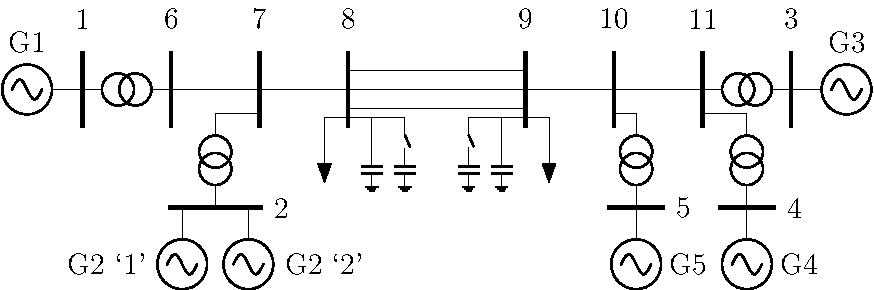
\includegraphics[width=\figW\linewidth]{../../models/sixMachine/sixMachine}\vspace{-.5em}
	\caption{Six Machine System Model.}
	\label{system}		 
\end{figure}%\vspace{-0em}


\paragraph{Additional Features} The behavior of PSDS to a 5\% load ramp on Bus 9 over 40 seconds can be matched fairly closely using LTD\footnote{LTD is using a 1 second time step while PSDS is using a 4.167 ms time step.}. Additionally, system inertia can be scaled\footnote{Hsys scaled by 75\%.} and effective droop can be taken into account\footnote{Generator 5 is un-governed.}. The effects of these optional simulation parameters on system frequency are shown in Figure \ref{featureComp}. 
\\

Note that the plotted theoretical steady state value was calculated using the ideal R values. If effective R values are used for the calculation, the calculated result matches the LTD Reff simulation result.

\begin{figure}[h!]
	\centering
	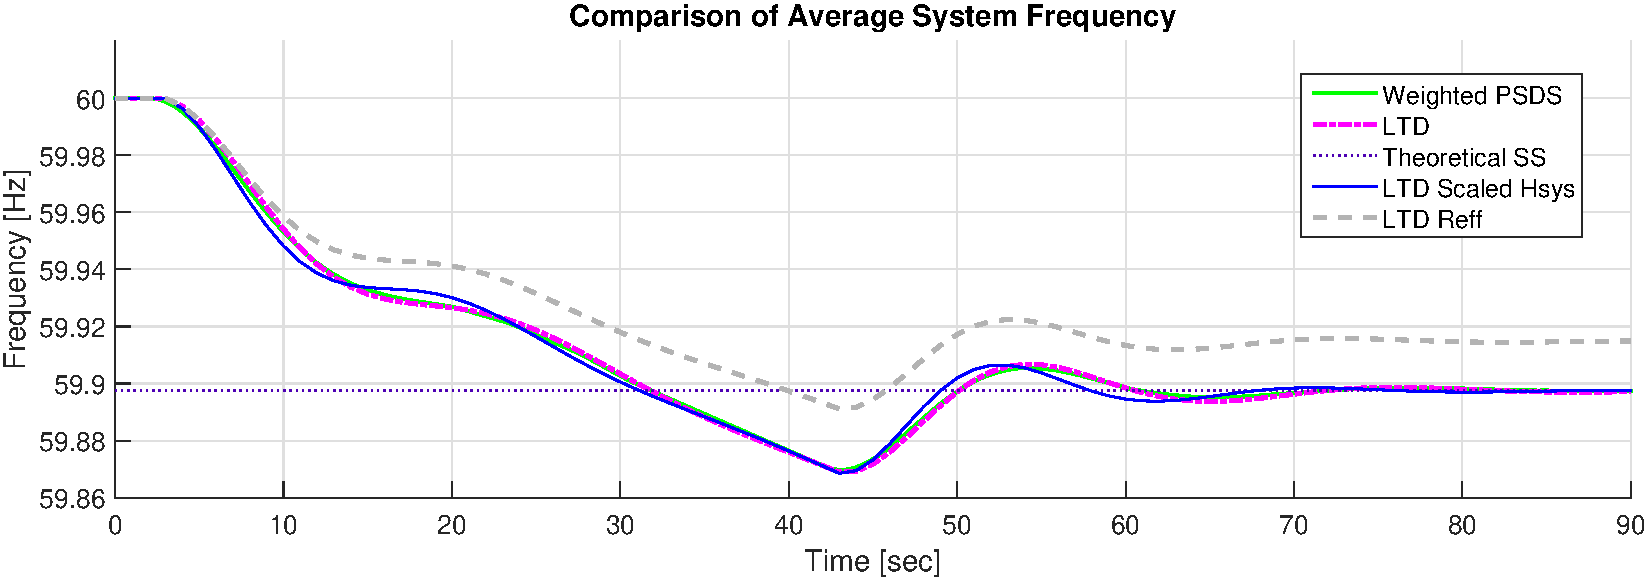
\includegraphics[width=\figW\linewidth]{HReffCompRamp}\vspace{-.5em}
	\caption{Comparison of LTD system frequency to PSDS weighted frequency.}
	\label{featureComp}		 
\end{figure}%\vspace{-0em}



\end{document}